\chapter{Introduction}
First, let's review a brief history of the origins of AI, its objectives and challenges met throughout the years. It is common to distinguish the old AI from the new, expliciting the breakthrough that happened in response to some \textit{failures} of the first type of AI.

\section{Old-fashioned AI}
\paragraph{Intelligence} It is first considered as a set of mental inferences, allowing the ability to make deductions, planning, mental simulations, reasoning, logics, and so on. Also, we distinguish rational intelligence from \textit{fake} intelligences, such as emotional intelligence, animal intelligence, embodied intelligence, collective intelligence. 
In other words, intelligence is described about IQ, chess, math, logical solving. All the rest is just skills.

\paragraph{The inferential engine} At this time, we're able to determine a general canvas and state the requirements of such an AI problem. Those are the following:
\begin{enumerate}
    \item Find the operators that can be applied: their pre-conditions need to match the current state of the world
    \item Select one the control strategy: in depth or in width, with heuristics or not
    \item Avoid looping
    \item Be able to backtrack
    \item Do that iteratively until you find the final state
\end{enumerate}
The solution of a planning problem is the sequence of operators. If several solutions are elligible, it is often the one having the shortest sequence of operators that will be optimal.


\paragraph{The failures} Man is embodied in his environment. He is a sophisticated sensori-motor process much before any cogitive process takes on. His perception is intrinsically and materially parallel. The sensori-motor processes essentially depends on
their biological grounding: parallel and adaptable.
The outside world is complex and to be able to cope with, a man requires an interface of similar complexity. But this complexity can be achieved by learning and experience rather than being handcrafted. Complex processes emerge from iterating simple mechanisms

\section{Today's AI}
Man possess 2 cognitive systems
\begin{enumerate}
    \item Parallel, automatic, unconscious, reflex, adaptable and very efficient. Based on neuronal hardware, for playing tennis, piano, becoming an expert, etc.
    \item Sequential, rigid, conscious and very laborious. Based on neuronal software, for playing chess, for testing IQ
\end{enumerate}
Man goes from one to the other in the cases of breakdowns in his
automatisms. Machine intelligence and human intelligence can be of different nature. For the machines today, recognizing a face is much more difficult than playing chess. But doesn’t Kasparov in part play chess like indeed we recognize a face?\\
~\\
We can describe the following trends:\\
AI $\rightarrow$ ALife \\
Software $\rightarrow$ Hardware \\
Cognitive Science $\rightarrow$ Biology
\paragraph{Summary} The animal hidden in each of us might be unavoidable on the road to intelligence. Our intellectual skills are embodied in our automatisms. They depart from there. In other words, don’t ever try to fully understand what a chair is without having ever sat in it. Also, a turn back is needed towards our biological interface with the outside world.

%%%%%%%%%%%%%%%%%%%%%%%%%%%%%%%%%%%%%%%%%%%%%%%%%%%%%%%
\chapter{State space search}
%%%%%%%%%%%%%%%%%%%%%%%%%%%%%%%%%%%%%%%%%%%%%%%%%%%%%%%
Search problems are described in terms of: \\
– An initial state. (e.g., initial chessboard, current positions of objects in world, current location) \\
– A target state.(e.g., winning chess position, target location) \\
– Some possible actions, that get you from one state to another. (e.g. chess move, robot action, simple change in location). \\
\linebreak
Search techniques systematically consider all possible action sequences to find a path from the initial to target state. The set of all possible states reachable from the initial state defines the search space. We can represent the search space as a tree.

\section{Exhaustive search algorithms}
We may use simple systematic search techniques, which try every possibility in systematic way. Those are referred to as brute force or blind techniques and include breadth first and depth first search among others.\\
\linebreak
The algorithms for breadth first and depth first search a very easy to implement. Both algorithms keep track of the list of nodes found. List is sometimes referred to as an agenda, but implemented using stack for depth first and a queue for breadth first.
\begin{algorithm}[caption={Breadth-first search.}, label={alg1}]
queue = {initial-state}
found = false
while queue not empty and not found
    remove the first node N from queue
    if N is a goal state
        found = true
    find all the successor nodes of N, and put them on the end of the queue
\end{algorithm}

\begin{algorithm}[caption={Depth-first search.}, label={alg2}]
stack = {initial-state}
found = false
while stack not empty and not found
    remove the first node N from stack
    if N is a goal state
        found = true
    find all the successor nodes of N, and put them on the end of the stack.
\end{algorithm}

\paragraph{Choice between algorithms} When is one technique more appropriate than the other? \\
– Shortest path? BF \\
– Is memory a problem? DF \\
– Need to find the solution quickly? It depends on the structure of the search tree. To avoid long paths in DF search, define a depth limit. To find shortest path quickly, change DF search to iterative deepening.

\paragraph{Extensions to basic algorithm} What if there are loops (i.e., we are search a graph)? How do you avoid (virtually) driving round and round in circles? Algorithm needs to keep track of which nodes have already been explored, and avoids redoing these nodes.

\begin{algorithm}[caption={Variation of depth-first search.}, label={alg3}]
stack = {initial-state}
visited = $\emptyset$
found = false
while stack not empty and not found
    remove the first node N from stack
    if N $\notin$ visited
        visited = visited $\cup$ N
        if N is a goal state
            found = true
        find all the successor nodes of N, and put them on the end of the stack.
\end{algorithm}


\section{Heuristic search algorithms}
Depth first and breadth first search turn out to be too inefficient for really complex problems. Instead, we turn to “heuristic search” methods, which do not
search the whole search space, but focus on promising areas.\\
\linebreak 
To identify promising areas, we need an \textbf{evaluation function}. The evaluation function scores a node in the search tree on how close it is to the goal/target state.
\begin{algorithm}[caption={Hill climbing.}, label={alg4}]
current_state = initial_state
while current_state $\neq$ goal-state $\vee$ no change in current state
    get the successors of current_state
    evaluate the successors and assign them a score
    if one of the successors is better than current_state
        then set the new-current state to be the successor with the best score
\end{algorithm}
This algorithm avoids loop, but may halt without success in local maximum.

\begin{algorithm}[caption={Best first search.}, label={alg5}]
agenda = {initial_state}
found = false
while agenda $\neq \emptyset$ and not found
    remove the best node N from agenda
    if N is a goal state
        found = true
    find all successor nodes of N, assign them a score, and put them on the agenda organised as a priority queue.
\end{algorithm}
Best first search algorithm works almost the same way as depth/breadth search algorithms, but we use a priority queue where nodes with high scores are taken of the queue first. Hence still exhaustive search and performance depends on the quality of the evaluation function.

\begin{algorithm}[caption={A*.}, label={alg6}]
agenda = {initial_state}
found = false
while agenda $\neq \emptyset$ and not found
    remove best node N from agenda
    if N is a goal state
        found = true
    for s in all successor nodes of n
        s.score  = cost(initial_state, s) + cost(s, goal_state)
    put all successor nodes on the agenda organised as a priority queue
\end{algorithm}
This algorithm is basically an extension of the best-first search, taking the total path length into account. The score is based on the predicted total path “cost”, that is, a sum of the cost/distance from initial to current node, and the predicted cost/distance to target node.\\
\linebreak
In BF search (if the cost of traversing a link is the same), the solution with the lowest cost will be found first, but it may take time. In DF search, a solution can be found quickly, yet it may not be a very good one. The A* algorithm finds a cheap solution quickly.

\paragraph{Summary} General search methods can be used to solve
complex problems, which are formulated in terms of initial and target state, and the primitive actions that take you from one state to next. Also, one may need to use heuristic search for complex problems, as search space can be too large.


\chapter{Concept learning}
This section describes the functioning of algorithms able to learn from examples, determine version spaces and implement the candidate elimination algorithm.
\section{The inductive learning hypothesis} Any hypothesis found to approximate the target function well over a sufficiently large set of training examples will also approximate the target function well over other unobserved examples.

\paragraph{An example problem} For the \textit{EnjoySport} problem, the canvas is the following (refer to the slides for the full problem description).\\
\textbf{Given:}\\
- Instances $X$ (e.g. possible days described by attributes Sky, AirTemp, Humidity, etc),\\
- Target function $c$: EnjoySport : $X \rightarrow {0, 1}$,\\
- Hypotheses $H$: conjunctions of literals (e.g. $\langle$?, Cold, High, ?, ?, ? $\rangle$),\\
- Training examples $D$: positive and negative examples of the target function $\langle x_1, c(x_1) \rangle, ..., \langle x_m, c(x_m) \rangle$.\\
\textbf{Determine:}\\
A hypothesis $h$ in H such that $h(x) = c(x)$ ~ $\forall x \in D$.


\begin{algorithm}[caption={Find-S.}, label={alg7}]
$h$ = most specific hypothesis in $H$
for each positive training instance $x$
    for each attribute constraint $a_i$ in $h$
        if $a_i$ satisfied by $x$
            do nothing
        else 
            replace $a_i$ by the next more  general constraint satisfied by $x$
return $h$
\end{algorithm}
This algorithm seeks the most restrictive (i.e most \textit{specific}) hypothesis that fits all the positive examples (negatives are ignored). This algorithm shows a few drawbacks:\\
- Can't tell whether it has learned concept\\
- Can't tell when training data inconsistent\\
- Picks a maximally specific $h$ (why?)\\
- Depending on $H$, there might be several!

\section{Version spaces} A hypothesis $h$ is consistent with a set of
training examples $D$ of target concept $c$ if and only if $h(x) = c(x)$ for each training example $\langle x, c(x) \rangle$ in $D$.
\begin{equation*}
    Consistent(h, D) \equiv (\forall \langle x, c(x) \rangle \in D) ~ h(x) = c(x) 
\end{equation*}
The version space, $VS_{H,D}$, with respect to hypothesis space $H$ and training examples $D$, is the subset of hypotheses from $H$ consistent with all training examples in $D$.
\begin{equation*}
    VS_{H, D} \equiv  \{ h \in H ~|~ Consistent(h, D) \}
\end{equation*}


\begin{algorithm}[caption={List-then-eliminate.}, label={alg8}]
$VS \leftarrow$  list containing every hypothesis in $H$
for each training example $\langle h(x), c(x) \rangle$
    remove from $VS$ any hypothesis $h$ for which $h(x) \neq c(x)$
return $VS$
\end{algorithm}

\paragraph{Representing version spaces} The general boundary, $G$, of version space $VS_{H, D}$ is the set of its maximally \textbf{general} members. The specific boundary, $S$, of $VS_{H, D}$ is the set of its maximally \textbf{specific} members. Every member of the version space lies between these boundaries:
\begin{equation*}
    VS_{H, D} = \{ h \in H ~|~ g \geq h \geq s,~ \forall s \in S,~ g \in G \}
\end{equation*}
where $x \geq y$ means $x$ is more general or equal to $y$.


\begin{algorithm}[caption={Candidate elimination.}, label={alg9}]
$G \leftarrow$ maximally general hypotheses in $H$
$S \leftarrow$ maximally specific hypotheses in $H$
for each training example $d$
    if $d$ is a positive example
        remove from $G$ any hypothesis inconsistent with $d$
        for each hypothesis $s \in S$ inconsistent with $d$
            $S \leftarrow S \setminus s$
            $S \leftarrow S \cup \{ all minimal generalizations h of s | Consistent(h, d) \wedge  some member of G is more general than h \}$
            $S \leftarrow S \setminus \{ h ~|~ h > s ~ \forall h \in H,~ s \in S \}$
    if $d$ is a negative example 
        remove from S any hypothesis inconsistent with d
        for each hypothesis g in G that is not consistent with d
            $G \leftarrow G \setminus g$
            $G \leftarrow G \cup \{all minimal specializations h of g | Consistent(h, d) \wedge some member of S is more specific than h \}$
            $G \leftarrow G \setminus \{ h ~|~ h < g ~ \forall h \in H,~ g \in G \}$

\end{algorithm}
To-do: notes on this algorithm

\section{Bias}
So far, we have three types of learners with different biases:
\begin{enumerate}
    \item Rote learner: store examples, classify $x$ if and only if it matches previously observed example.
    \item Version space candidate elimination algorithm
    \item Find-S algorithm
\end{enumerate}
\paragraph{An unbiased learner} The idea is to choose and $H$ that expresses every teachable concept (i.e. $H$ is the power set of $X$, $2^X$).

\paragraph{Inductive bias} Let's consider concept learning algorithm $L$, a set of instances $X$, a target concept $c$, a set of training examples $D_c = \{ \langle x, c(x) \rangle \}$. Let $L(x_i, D_c)$ denote the classification assigned to the instance $x_i$ by $L$ after training on data $D_c$.\\
\linebreak The inductive bias of $L$ is any minimal set of assertions $B$ such that for any target
concept $c$ and corresponding training
examples $D_c$:
\begin{equation*}
(\forall x_i \in X) [ ( B \wedge D_c \wedge x_i) \vdash L(x_i, D_c)]
\end{equation*}
where $A \vdash B$ means $A$ logically entails $B$

\begin{figure}[h]
    \centering
    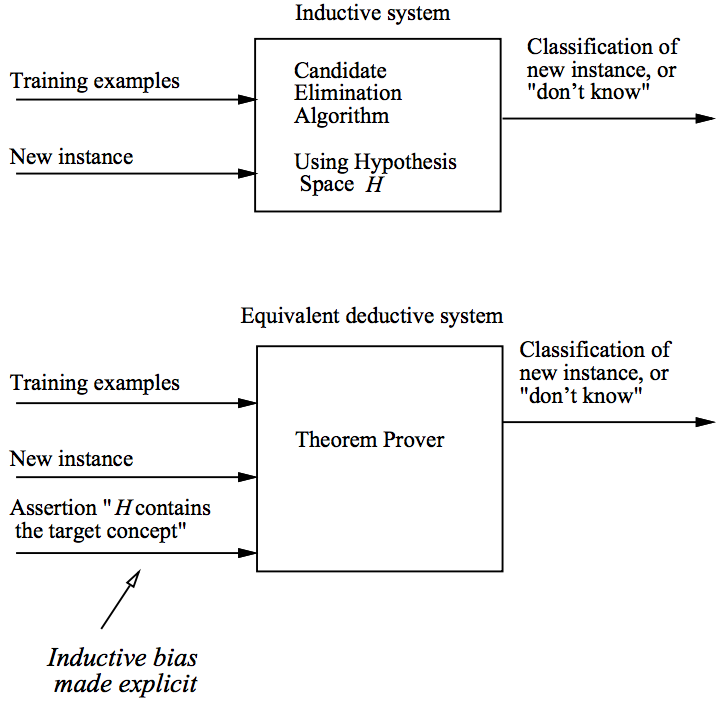
\includegraphics[width=0.7\linewidth]{img/inductivebias}
\end{figure}

\paragraph{Summary Points}
\begin{enumerate}
    \item Concept learning as search through $H$
    \item General-to-specific ordering over $H$
    \item Version space candidate elimination algorithm
    \item $S$ and $G$ boundaries characterize learner's uncertainty
    \item Learner can generate useful queries
    \item Inductive leaps possible only if learner is biased
    \item Inductive learners can be modelled by equivalent deductive systems
\end{enumerate}